%================================================================
\section{Results}\label{sec:results}
% Present results and give a critical discussion of my work in 
% the context of other work. Relate the work to previous studies, 
% and make sure the results are reproducible. Include information 
% in figure captions such that they can give the reader enough to 
% understand the main gist of the report.
%================================================================
\subsection{Synthetic data analysis}\label{ssec:synthetic_data}
I generated two synthetic data set, one of which included stochastic noise, from the Franke function in Equation \eqref{eq:franke_function}. To keep the initial analysis efficient and interpretable, I used $50 \times 50$ data points and noise $\epsilon \sim \mathcal{N}(0, 0.1)$ with less variance than suggested in the project description. 

\subsubsection{Ordinary Least Squares}\label{sssec:ols}
I performed an OLS regression analysis up to a fifth polynomial degree, and computed the MSE and R$^{2}$-score for performance on both data set. The model's coefficients are shown in Figure \ref{fig:ols_beta_smooth} and Figure \ref{fig:ols_beta}. The MSE and R$^{2}$-score is shown in Figure \ref{fig:ols_error_smooth} and Figure \ref{fig:ols_error}.

\begin{figure}
    \centering
    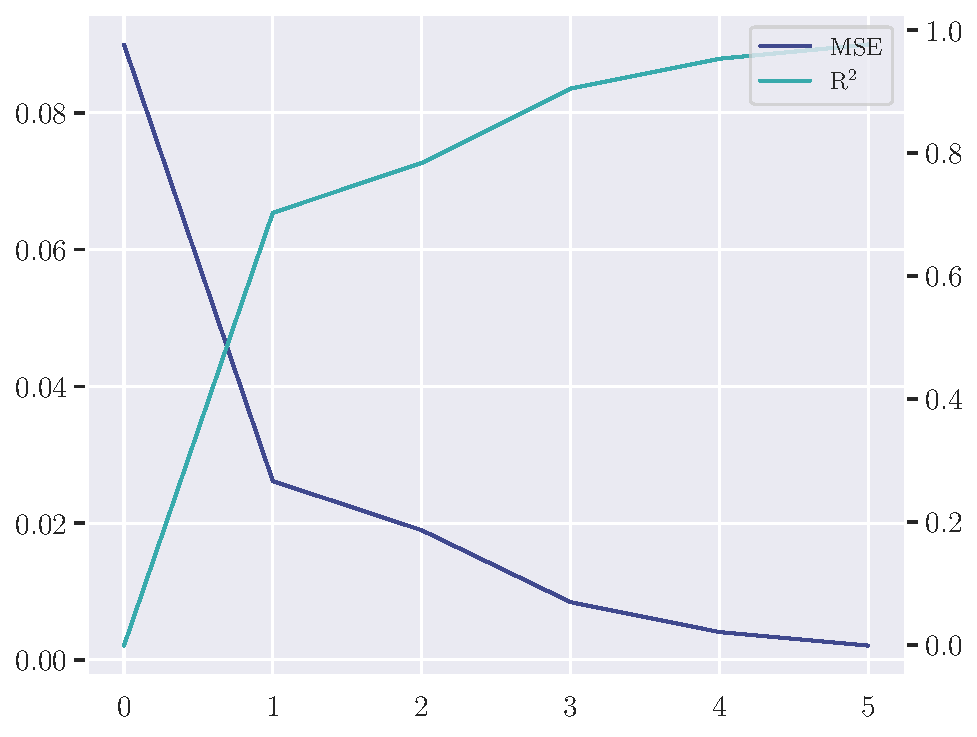
\includegraphics[width=0.9\linewidth]{project-1/latex/figures/ols_error.pdf}
    \caption{MSE and R$^{2}$-score computed on test data, as a function of the polynomial degree of the input features. The function data was generated without stochastic noise.}
    \label{fig:ols_error}
\end{figure}

\begin{figure}
    \centering
    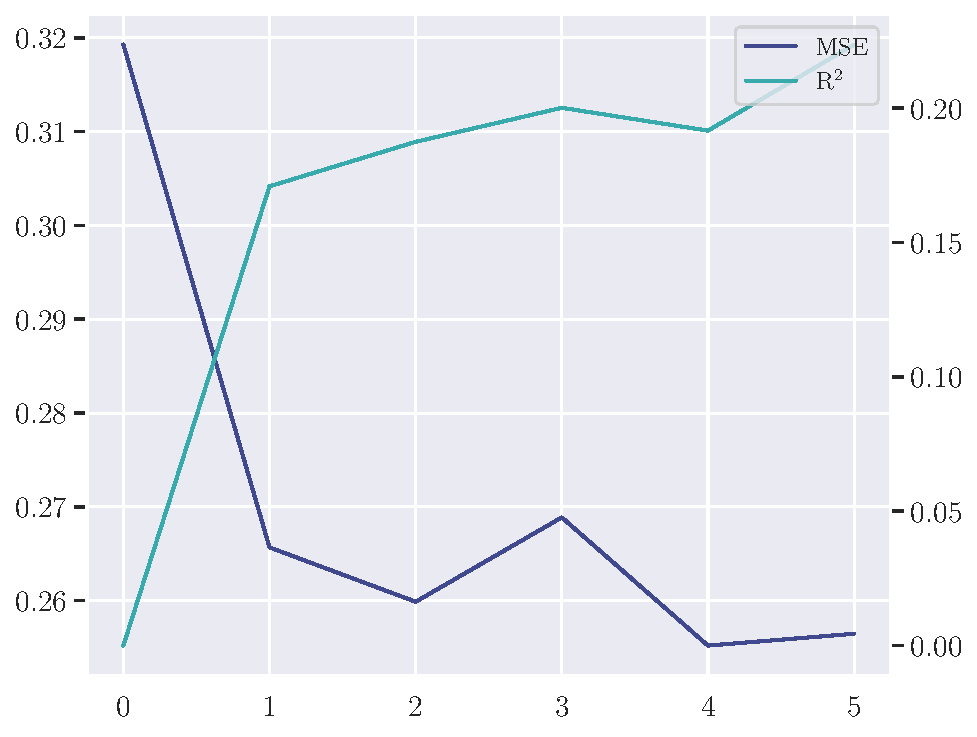
\includegraphics[width=0.9\linewidth]{project-1/latex/figures/ols_error_noisy.pdf}
    \caption{MSE and R$^{2}$-score computed on test data, as a function of the polynomial degree of the input features. The function data includes stochastic noise $\epsilon \in \mathcal{N}(0, 1)$.}
    \label{fig:ols_error_noisy}
\end{figure}

When noise is included in the function data, the error increases for all polynomial degrees. Since the R$^{2}$-score determines how large a proportion of the variance in the dependent variable is explained by the independent variable, it seems the model only explains the input features.

Looking at $\beta$-values for the model fitting the function data without noise in Figure \ref{fig:ols_beta}, and the function data with noise Figure \ref{fig:ols_beta_noisy}. As the polynomial degree increase, the absolute values of $\beta$ increase. However, both the absolute values and variance between each $\beta_{i}$ increase when noise is included in the function.  
\begin{figure}
    \centering
    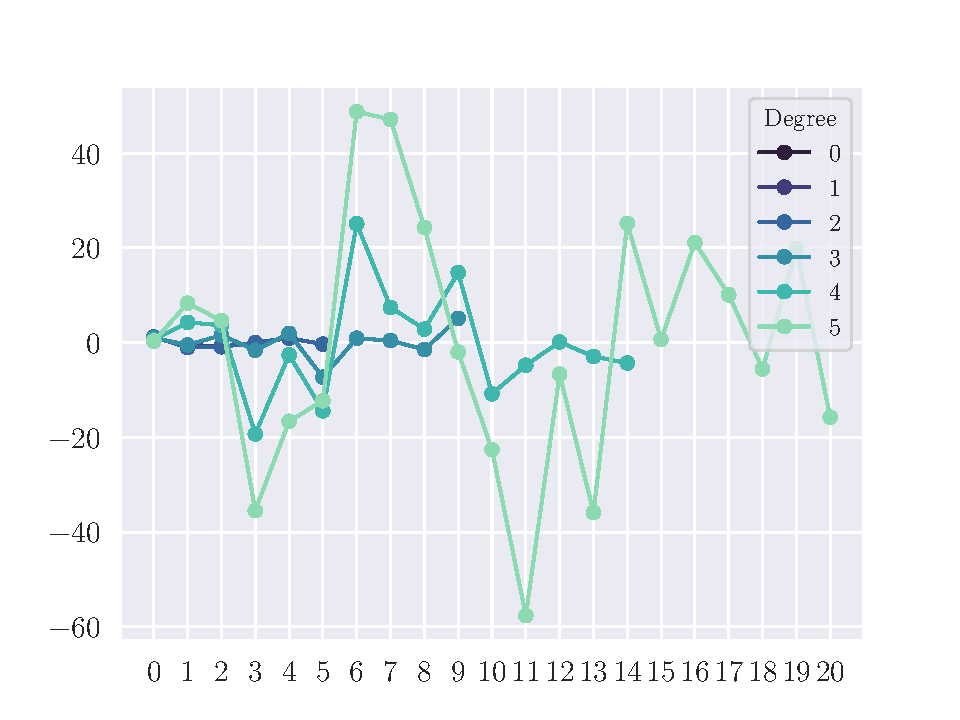
\includegraphics[width=0.9\linewidth]{project-1/latex/figures/ols_beta.pdf}
    \caption{The figure shows beta values for different polynomial degree.}
    \label{fig:ols_beta}
\end{figure}

\begin{figure}
    \centering
    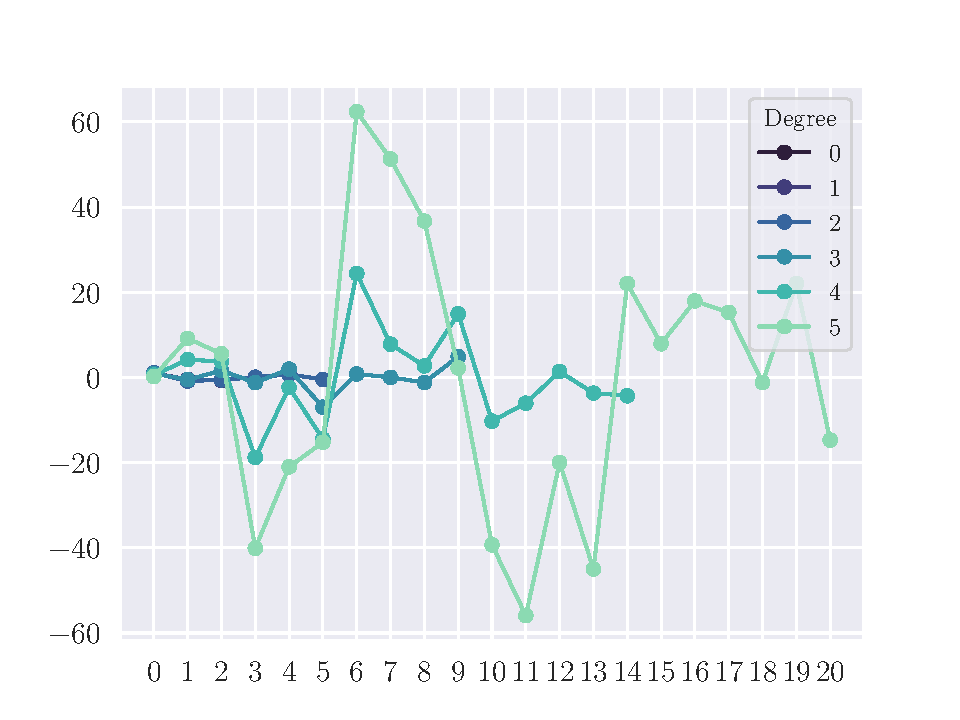
\includegraphics[width=0.9\linewidth]{project-1/latex/figures/ols_beta_noisy.pdf}
    \caption{The figure shows beta values for different polynomial degree, when the function includes noise.}
    \label{fig:ols_beta_noisy}
\end{figure}

I continued the regression analysis with data from the Franke function which included noise.